%%%%%%%%%%%%%%%%%%%%%%%%%%%%%%%%%%%%%%%%%%%%%%%%%
%================================================
% Numerical results: verification of the monolithic FE formulation against the
% Green-function theory of Section \ref{sec:discrete_lattice}, configuration A,
% vertical section (tests L1-1, L1-2, L1-3 of the verification test matrix).
% Source: HydroElasticFEM_xxx2026.jl (L1-1: commit 1ea6a27, L1-2: c87174c,
% L1-3: 2026-10-16; L1-3b, L1-4, L1-5, L1-6, L1-8: commits dff545a, b7965bb,
% 50b6643, 1cf39c4, 2026-10-23), records data/sims/L1-*, figures plots/L1-*.
% Figures expected in figures/L1_*.png.
%================================================
\section{Numerical Results}\label{sec:numerical_results}

The formulation of Section~\ref{sec:numerical_formulation} is implemented in the Julia package HydroElasticFEM.jl, built on the Gridap finite element library \cite{badia2020gridap,verdugo2022software}, following \cite{colomes2023monolithic,agarwal2024dynamic}. The weak forms are written almost verbatim in Gridap's high-level syntax, which supports integration on entities of four different dimensions: the fluid cells $\Omega_h$, the surface facets $\Gfh$ and $\Gmh$ (on which the elevation spaces are traces of the fluid mesh), the structural skeleton $\Lmh$ of the C/DG terms, and the attachment points $\xvec_i$, where Dirac measures evaluate $\eta_h$ and $u_h$. The resonator amplitudes are global scalar unknowns of the multi-field space $\mathcal{X}_h$. The frequency-domain system \eqref{eq:algebraic_system} is solved with a sparse direct solver, with one factorisation per frequency.

{\color{red}
\subsection{Verification against the Green-function theory: infinite structure in the vertical section}\label{subsec:num_verification_A}

The finite element formulation of Section~\ref{sec:numerical_formulation} is verified here against the exact results of Section~\ref{sec:discrete_lattice} for an infinite structure, configuration~A, in the vertical section. The bare host is characterised by its symbol $\mathcal{D}_0$, equation~\eqref{eq:host_symbol}, and by the Green function~\eqref{eq:lat_green_1d}; a single resonator enters only through the combination $1/\alpha-G(0)$ of equation~\eqref{eq:single_force}. The verification therefore proceeds in three steps, each relying on the previous one: (i) the discrete propagating wavenumber and the discrete Green function of the bare host (Section~\ref{subsubsec:num_L1_1}); (ii) the radiative width $\gamma_r$ and the energy flux, which normalise every reflection, transmission and absorption coefficient computed from finite element wave amplitudes (Section~\ref{subsubsec:num_L1_2}); and (iii) the scattering by a single resonator, including the renormalised resonance, the half-power bandwidth and critical coupling (Section~\ref{subsubsec:num_L1_3}).

\subsubsection{Numerical setup}\label{subsubsec:num_setup_A}

\paragraph{Host and resonator.} All tests use the plate and fluid parameters of Table~\ref{tab:dispersion_test_parameters}: $\rho=1000~\si{\kilogram\per\meter\cubed}$, $g=9.8~\si{\meter\per\second\squared}$, $H=10~\si{\meter}$, $m_\rho=0.01~\si{\meter}$, $C_\rho=0.49~\si{\meter\tothe{5}\per\second\squared}$, with $T_\rho=0$ and $T_\rho=9.8~\si{\meter\cubed\per\second\squared}$, and no material damping in the plate ($\tau=\tau_b=0$). The resonator of Section~\ref{subsubsec:num_L1_3} has $m_{\rho,r}=0.01~\si{\meter\squared}$ per unit width and $\omega_r=10~\si{\radian\per\second}$. At $\omega=10~\si{\radian\per\second}$ the plate wavelength is $\lambda_0=2\pi/k_0=2.29~\si{\meter}$ ($T_\rho=0$) and $3.26~\si{\meter}$ ($T_\rho=9.8~\si{\meter\cubed\per\second\squared}$), the flexural roots decay over $0.37$ and $0.23~\si{\meter}$, and the slowest evanescent fluid mode, $k_1\simeq\mathrm{i}\pi/H$ in equation~\eqref{eq:green_function}, over $1/\operatorname{Im}k_1=6.3~\si{\meter}\approx2H/\pi$.

\paragraph{Computational domain.} The infinite structure is represented by a channel of depth $H$ whose free surface is entirely covered by the plate and which is closed by rigid walls (Figure~\ref{fig:num_channel_A}). Outgoing waves are absorbed by sponge layers of length $6\lambda_0$ at both ends, in which the bending stiffness is made viscoelastic, $C_\rho\to C_\rho(1-\mathrm{i}s(x))$, i.e.\ the structural damping term of equation~\eqref{eq:Bilinear_freq} with a position-dependent loss factor $\omega\tau_b(x)=s(x)$ rising quadratically from $0$ to $3$. These sponges act on bending only: they absorb short waves well but not long waves (at $\omega\le1~\si{\radian\per\second}$ the waves are fully reflected), and they do not damp the evanescent fluid modes, which carry no energy flux. Three precautions make the results independent of the truncation:
\begin{enumerate}
    \item every source and resonator is at least $5/\operatorname{Im}k_1$ (about $32~\si{\meter}$ at $\omega=10~\si{\radian\per\second}$) from the sponges, so that the evanescent field reflected by the sponges and walls is reduced by $\mathrm{e}^{-10}$;
    \item the channel length is $L=(n+\tfrac14)\lambda_0$, $n\in\mathbb{N}$, midway between the resonances $L=n\lambda_0/2$ of the closed channel, which would otherwise be excited at low frequency where the sponges are transparent;
    \item all coefficients are extracted with relations that are exact for any amount of wave reflection from the ends (see the post-processing below).
\end{enumerate}

\begin{figure}[t]
    \centering
    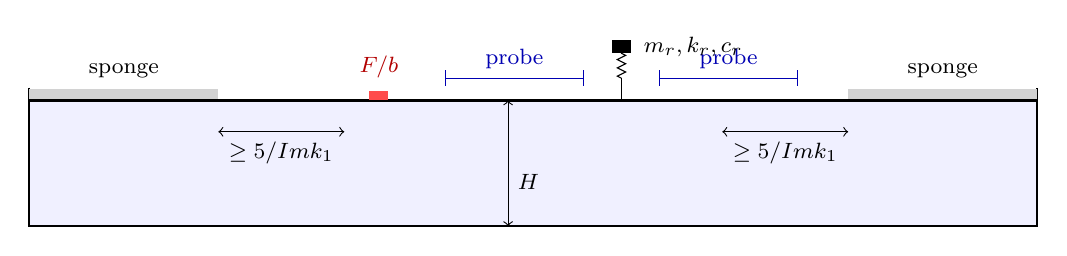
\begin{tikzpicture}[x=0.8cm,y=0.8cm,font=\footnotesize]
        % fluid and walls
        \fill[blue!6] (0,0) rectangle (16,-2);
        \draw[thick] (0,0.2) -- (0,-2) -- (16,-2) -- (16,0.2);
        % sponges
        \fill[gray!35] (0,0) rectangle (3,0.18);
        \fill[gray!35] (13,0) rectangle (16,0.18);
        \node[above] at (1.5,0.2) {sponge};
        \node[above] at (14.5,0.2) {sponge};
        % plate
        \draw[very thick] (0,0) -- (16,0);
        % buffers
        \draw[<->] (3,-0.5) -- (5,-0.5) node[midway,below] {$\ge 5/\operatorname{Im}k_1$};
        \draw[<->] (11,-0.5) -- (13,-0.5) node[midway,below] {$\ge 5/\operatorname{Im}k_1$};
        % source
        \fill[red!70] (5.4,0) rectangle (5.7,0.15);
        \node[above,red!70!black] at (5.55,0.2) {$F/b$};
        % probes
        \draw[|-|, blue!70!black] (6.6,0.35) -- (8.8,0.35) node[midway,above] {probe};
        \draw[|-|, blue!70!black] (10.0,0.35) -- (12.2,0.35) node[midway,above] {probe};
        % resonator
        \draw (9.4,0) -- (9.4,0.35);
        \draw[decorate,decoration={zigzag,amplitude=1.5pt,segment length=3pt}] (9.4,0.35) -- (9.4,0.75);
        \fill (9.25,0.75) rectangle (9.55,0.95);
        \node[right] at (9.6,0.85) {$m_r,k_r,c_r$};
        % depth
        \draw[<->] (7.6,0) -- (7.6,-2);
        \node[right] at (7.6,-1.3) {$H$};
    \end{tikzpicture}
    \caption{Configuration-A channel used for the verification (not to scale): plate over the whole free surface, sponge layers in front of rigid walls, patch source of width $b$, probe windows on which the wave amplitudes are fitted, and (Section~\ref{subsubsec:num_L1_3}) one resonator between the probes. In Sections~\ref{subsubsec:num_L1_1} and~\ref{subsubsec:num_L1_2} the probes are placed on both sides of the source.}
    \label{fig:num_channel_A}
\end{figure}

\paragraph{Forcing.} The waves are generated by a uniform pressure $F/b$ applied over a patch of two plate elements, $b=2h$, which enters the linear form as $(F/b,u)_{\Gamma_m}$. The response of the bare host to this load is known exactly outside the patch,
\begin{equation}\label{eq:num_patch_green}
    G_b(x)=\mathrm{i}\sum_m\operatorname{sinc}\!\Big(\frac{k_mb}{2}\Big)\frac{\mathrm{e}^{\mathrm{i}k_m|x|}}{\mathcal{D}_0'(k_m)},\qquad |x|\ge b/2,
\end{equation}
which reduces to equation~\eqref{eq:lat_green_1d} as $b\to0$. The residue series includes the propagating root, the complex flexural pair and $100$ evanescent roots, enough to evaluate $G(0)$ to a relative accuracy of $10^{-11}$.

\paragraph{Discretisation.} The fluid potential and the plate deflection are approximated with Lagrange polynomials of degree $p\in\{2,3\}$ on a structured mesh, with the C/DG treatment of the plate bending term of Section~\ref{sec:numerical_formulation} (penalty parameter $\gamma=6$). The horizontal element size is $h=\lambda_0/n_\lambda$, with $n_\lambda$ elements per plate wavelength: $n_\lambda\in\{20,40,80\}$ for $p=2$ and $n_\lambda\in\{10,20,40\}$ for $p=3$. Vertically, the mesh is graded geometrically towards the plate, with a top cell of size $h/2$ and a growth ratio bounded by $1+0.2\,(20/n_\lambda)$. Reducing the growth ratio with $h$ makes every cell, down to the bottom, shrink with the mesh size; with a fixed ratio, the cells near the bottom keep their size under refinement, which limited the observed order to $1.25$ at frequencies where the wave reaches the bottom ($k_0H\approx1$--$4$). The largest problems have $1.2\times10^6$ degrees of freedom.

\paragraph{Post-processing.} The plate deflection is sampled on probe windows of three wavelengths and fitted, in the least-squares sense, by
\begin{equation}\label{eq:num_wave_fit}
    \widehat{\eta}_h(x)\simeq A^+\mathrm{e}^{\mathrm{i}k_h(x-x_\mathrm{ref})}+A^-\mathrm{e}^{-\mathrm{i}k_h(x-x_\mathrm{ref})}+\sum_{n=1}^{6}\Big(c_n^+\mathrm{e}^{\mathrm{i}k_n(x-x_a)}+c_n^-\mathrm{e}^{\mathrm{i}k_n(x_b-x)}\Big),
\end{equation}
where $[x_a,x_b]$ is the probe window, $x_\mathrm{ref}$ the source or resonator position, and $k_n$ the flexural pair and the four slowest evanescent roots. The wavenumber $k_h$ is the discrete one, fitted on the field rather than set to $k_0$: with $k_0$ the dispersion error of the discretisation would accumulate in the phase of the amplitudes over the distance to $x_\mathrm{ref}$. Fitting both directions separates the outgoing waves from those returning from the sponges; the source is transparent to the returning waves, so the wave radiated towards one side is the outgoing amplitude on that side minus the incoming amplitude on the other. The accuracy of each quantity $Q_h$ is measured by its relative error against the exact value, $e(Q)=|Q_h/Q-1|$, and the observed order of convergence between the two finest meshes is $\log(e_1/e_2)/\log 2$.

The C/DG plate discretisation converges at order $p-1$ in the energy norm, so that smooth functionals of the solution, such as the wavenumber, the radiated amplitude or the resonance frequency, are expected to converge at order $2(p-1)$. A test is passed when the error on the finest mesh is below $10^{-3}$ for every quantity, and, for $p=2$, when the observed order is at least $2(p-1)-0.3=1.7$. For $p=3$ the errors on the finest meshes reach values between round-off and $10^{-6}$, at which the observed order is no longer a meaningful measure of the discretisation; it is reported but not used as a criterion.

\subsubsection{Bare host: dispersion and Green function}\label{subsubsec:num_L1_1}

\paragraph{Test description.} A patch force $F$ is applied at the centre of the channel without resonators, and three quantities are compared with the theory: (i) the discrete propagating wavenumber $k_h$, fitted on both sides of the source, against the root $k_0$ of equation~\eqref{eq:host_symbol}; (ii) the radiative width obtained from the radiated amplitude $A$, $\gamma_h=A/(\mathrm{i}F\operatorname{sinc}(k_0b/2))$, against $\gamma_r=\operatorname{Im}G(0)=1/\mathcal{D}_0'(k_0)$, equation~\eqref{eq:lat_green_1d}; and (iii) the near field between the patch edge and one wavelength from the source, after subtraction of the waves returning from the sponges, against $FG_b(x)$, equation~\eqref{eq:num_patch_green}, with real and imaginary parts compared separately. The real part of $G$ sets the renormalised resonance of a resonator, equation~\eqref{eq:renorm_single}, and the imaginary part its radiation, equation~\eqref{eq:ImG}. The test is performed first at $\omega=10~\si{\radian\per\second}$ ($T_\rho=0$) on a wide range of meshes, and then for $30$ frequencies logarithmically spaced in $[0.3,15]~\si{\radian\per\second}$ and both pre-tensions. In the frequency sweep only the far-field quantities (i) and (ii) are considered: at low frequency the element size, about $10~\si{\meter}$ at $\omega=0.3~\si{\radian\per\second}$, is much larger than the decay lengths of the near field, which do not scale with the wavelength.

\paragraph{Results.} Table~\ref{tab:num_L1_1} and Figure~\ref{fig:num_L1_1_convergence} show the convergence at $\omega=10~\si{\radian\per\second}$. With $p=2$ all four quantities converge at order $2.0$ from $10$ elements per wavelength on, with the wavenumber about four times more accurate than the radiated amplitude and the near field. With five elements per wavelength the solution is not yet in the asymptotic range: the radiative width is in error by $28\%$. With $p=3$ the errors are three to five orders of magnitude smaller at equal mesh size and fall below $10^{-6}$ with $40$ elements per wavelength, where the real part of the near field and the radiative width level off at about $10^{-6}$ and $2.5\times10^{-7}$, respectively. The frequency sweep (Figures~\ref{fig:num_L1_1_sweep_k} and~\ref{fig:num_L1_1_sweep_gamma}) confirms this picture over the whole range: with $p=2$ the observed order of the wavenumber error is close to $4$ at low frequency, where the bending term is negligible and the wave is essentially a long gravity wave under an inertial plate, and decreases to the order $2$ of the C/DG bending discretisation above $\omega\approx3~\si{\radian\per\second}$, where bending controls the dispersion. The errors increase with frequency and are smaller with pre-tension; on the finest meshes they remain below $1.0\times10^{-4}$ (wavenumber) and $4.1\times10^{-4}$ (radiative width) for $p=2$, and below $2.5\times10^{-8}$ and $7\times10^{-7}$ for $p=3$. At $\omega\le1~\si{\radian\per\second}$ the sponges reflect all the incident energy, and the extraction of the amplitudes, which is exact under reflection, still gives errors between $10^{-10}$ and $10^{-6}$.

\begin{table}[t]
    \centering
    \caption{Bare host at $\omega=10~\si{\radian\per\second}$, $T_\rho=0$: relative errors of the discrete wavenumber, of the radiative width obtained from the far field, and of the real and imaginary parts of the near field, against $k_0$, $\gamma_r=1/\mathcal{D}_0'(k_0)$ and $FG_b(x)$.}
    \label{tab:num_L1_1}
    \footnotesize
    \begin{tabular}{rrrcccc}
        \hline
        $p$ & $n_\lambda$ & DOFs & $k_h$ & $\gamma_h$ & $\operatorname{Re}\widehat{\eta}_h$ & $\operatorname{Im}\widehat{\eta}_h$ \\
        \hline
        2 & 5  & 6\,480   & $6.3\times10^{-3}$ & $2.8\times10^{-1}$ & $8.2\times10^{-2}$ & $1.5\times10^{-1}$ \\
        2 & 10 & 19\,368  & $6.2\times10^{-3}$ & $2.3\times10^{-2}$ & $3.0\times10^{-2}$ & $3.5\times10^{-2}$ \\
        2 & 20 & 67\,662  & $1.5\times10^{-3}$ & $6.4\times10^{-3}$ & $8.0\times10^{-3}$ & $9.2\times10^{-3}$ \\
        2 & 40 & 251\,238 & $3.9\times10^{-4}$ & $1.6\times10^{-3}$ & $2.1\times10^{-3}$ & $2.3\times10^{-3}$ \\
        2 & 80 & 966\,150 & $9.7\times10^{-5}$ & $4.1\times10^{-4}$ & $5.2\times10^{-4}$ & $5.7\times10^{-4}$ \\
        3 & 5  & 13\,961  & $5.2\times10^{-4}$ & $7.4\times10^{-3}$ & $2.8\times10^{-3}$ & $2.5\times10^{-3}$ \\
        3 & 10 & 42\,350  & $9.0\times10^{-6}$ & $8.3\times10^{-5}$ & $1.7\times10^{-4}$ & $6.2\times10^{-5}$ \\
        3 & 20 & 149\,792 & $4.9\times10^{-7}$ & $7.2\times10^{-6}$ & $1.2\times10^{-5}$ & $3.4\times10^{-6}$ \\
        3 & 40 & 560\,396 & $4.3\times10^{-9}$ & $2.5\times10^{-7}$ & $1.1\times10^{-6}$ & $2.9\times10^{-7}$ \\
        \hline
    \end{tabular}
\end{table}

\begin{figure}[t]
    \centering
    \begin{subfigure}{0.49\linewidth}
        \includegraphics[width=\linewidth]{figures/L1_1_convergence_p2.png}
        \caption{$p=2$}
    \end{subfigure}
    \begin{subfigure}{0.49\linewidth}
        \includegraphics[width=\linewidth]{figures/L1_1_convergence_p3.png}
        \caption{$p=3$}
    \end{subfigure}
    \caption{Bare host at $\omega=10~\si{\radian\per\second}$, $T_\rho=0$: relative errors against the number of elements per wavelength. Dashed: order $2(p-1)$.}
    \label{fig:num_L1_1_convergence}
\end{figure}

\begin{figure}[t]
    \centering
    \includegraphics[width=\linewidth]{figures/L1_1_sweep_k.png}
    \caption{Discrete wavenumber over the frequency range, $T_\rho=0$ (left) and $T_\rho=9.8~\si{\meter\cubed\per\second\squared}$ (right). Top: relative error $|k_h/k_0-1|$ for $p=2$ (black) and $p=3$ (blue) on three meshes (dotted, dashed, solid from coarse to fine). Bottom: observed order between the two finest meshes; dashed lines at $2(p-1)$.}
    \label{fig:num_L1_1_sweep_k}
\end{figure}

\begin{figure}[t]
    \centering
    \includegraphics[width=\linewidth]{figures/L1_1_sweep_gamma.png}
    \caption{Radiative width from the far field over the frequency range; layout as in Figure~\ref{fig:num_L1_1_sweep_k}.}
    \label{fig:num_L1_1_sweep_gamma}
\end{figure}

\subsubsection{Radiative width and energy flux}\label{subsubsec:num_L1_2}

\paragraph{Test description.} The radiative width $\gamma_r=\operatorname{Im}G(0)$ controls the critical damping and the absorption of every resonator configuration (Section~\ref{subsubsec:energy_flux_single}), and the energy flux~\eqref{eq:energy_flux} normalises the reflection, transmission and absorption coefficients. Both are verified by computing $\gamma_r$ in three independent ways from the same finite element solution of the bare host forced by the patch:
\begin{enumerate}
    \item \emph{far field}: from the radiated amplitudes, as in Section~\ref{subsubsec:num_L1_1};
    \item \emph{source patch}: in the non-dissipative case $\operatorname{Im}G(x)=\cos(k_0x)/\mathcal{D}_0'(k_0)$ for all $x$, equation~\eqref{eq:lat_green_1d}, so that the average of the patch response over the patch is $\operatorname{Im}\langle G_b\rangle=\operatorname{sinc}^2(k_0b/2)/\mathcal{D}_0'(k_0)$; the finite element average $\langle\widehat{\eta}_h\rangle$, computed by Gauss quadrature on the two patch elements and corrected for the waves returning from the sponges, gives $\gamma_h=\operatorname{Im}\langle\widehat{\eta}_h\rangle/(F\operatorname{sinc}^2(k_0b/2))$;
    \item \emph{work--flux balance}: the work done by the load, $P=\tfrac12\omega\operatorname{Im}(\overline{F}\langle\widehat{\eta}_h\rangle)$, which is equation~\eqref{eq:point_power} for a distributed load, is compared with the net flux $\tfrac14\omega\mathcal{D}_0'(k_0)\sum(|A_\mathrm{out}|^2-|A_\mathrm{in}|^2)$ through both probe windows, equation~\eqref{eq:energy_flux}; the error is $|P/P_\mathrm{flux}-1|$.
\end{enumerate}
The test is performed at $\omega\in\{2,5,10\}~\si{\radian\per\second}$ for both pre-tensions.

\paragraph{Results.} The three measures agree with each other and with $\gamma_r$ for all cases (Table~\ref{tab:num_L1_2} and Figure~\ref{fig:num_L1_2}). With $p=2$ they converge at order $2.0$ (observed orders $1.98$--$2.26$) to errors between $2.5\times10^{-6}$ and $4.1\times10^{-4}$ with $80$ elements per wavelength. The errors increase with frequency, as the bending term becomes dominant, and are two to eight times smaller with pre-tension. With $p=3$ all errors are below $3.3\times10^{-7}$ with $40$ elements per wavelength; at $\omega=10~\si{\radian\per\second}$ they reach the same level of $2$--$3\times10^{-7}$ found for the far field in Section~\ref{subsubsec:num_L1_1}. That the work done by the load equals the flux of the radiated waves to this accuracy confirms that equation~\eqref{eq:energy_flux}, derived from the Green function, is the energy flux of the discrete coupled fluid--structure system, and therefore that the reflection, transmission and absorption coefficients of Section~\ref{subsubsec:num_L1_3} are correctly normalised.

\begin{table}[t]
    \centering
    \caption{Radiative width: exact value $\gamma_r=1/\mathcal{D}_0'(k_0)$ (density-normalised symbol) and relative errors of the three finite element measures on the finest mesh ($n_\lambda=80$ for $p=2$, $40$ for $p=3$). $T_\rho$ in \si{\meter\cubed\per\second\squared}, $\omega$ in \si{\radian\per\second}.}
    \label{tab:num_L1_2}
    \footnotesize
    \begin{tabular}{rrcrccc}
        \hline
        $T_\rho$ & $\omega$ & $\gamma_r$ & $p$ & far field & source patch & work--flux \\
        \hline
        0   & 2  & 0.0415 & 2 & $5.9\times10^{-6}$ & $5.9\times10^{-6}$ & $5.9\times10^{-6}$ \\
            &    &        & 3 & $4.8\times10^{-9}$ & $4.8\times10^{-9}$ & $1.4\times10^{-9}$ \\
        0   & 5  & 0.0534 & 2 & $3.8\times10^{-4}$ & $3.8\times10^{-4}$ & $3.8\times10^{-4}$ \\
            &    &        & 3 & $1.6\times10^{-7}$ & $4.9\times10^{-8}$ & $5.7\times10^{-8}$ \\
        0   & 10 & 0.0186 & 2 & $4.1\times10^{-4}$ & $4.1\times10^{-4}$ & $4.1\times10^{-4}$ \\
            &    &        & 3 & $2.5\times10^{-7}$ & $2.1\times10^{-7}$ & $2.6\times10^{-7}$ \\
        9.8 & 2  & 0.0263 & 2 & $2.5\times10^{-6}$ & $2.5\times10^{-6}$ & $2.6\times10^{-6}$ \\
            &    &        & 3 & $1.4\times10^{-8}$ & $1.3\times10^{-8}$ & $2.4\times10^{-9}$ \\
        9.8 & 5  & 0.0224 & 2 & $4.9\times10^{-5}$ & $4.8\times10^{-5}$ & $4.9\times10^{-5}$ \\
            &    &        & 3 & $1.4\times10^{-7}$ & $9.9\times10^{-8}$ & $2.1\times10^{-9}$ \\
        9.8 & 10 & 0.0127 & 2 & $1.3\times10^{-4}$ & $1.3\times10^{-4}$ & $1.3\times10^{-4}$ \\
            &    &        & 3 & $3.1\times10^{-7}$ & $3.2\times10^{-7}$ & $2.8\times10^{-7}$ \\
        \hline
    \end{tabular}
\end{table}

\begin{figure}[t]
    \centering
    \includegraphics[width=\linewidth]{figures/L1_2_convergence_p2.png}\\
    \includegraphics[width=\linewidth]{figures/L1_2_convergence_p3.png}
    \caption{Radiative width from the far field, from the source patch and from the work--flux balance, for $p=2$ (top) and $p=3$ (bottom); colour: frequency, marker: pre-tension. Dashed: order $2(p-1)$.}
    \label{fig:num_L1_2}
\end{figure}

\subsubsection{Single resonator}\label{subsubsec:num_L1_3}

\paragraph{Test description.} One resonator ($m_{\rho,r}=0.01~\si{\meter\squared}$, $\omega_r=10~\si{\radian\per\second}$) is attached to the plate four and a half wavelengths downstream of the source, between two probe windows of three wavelengths placed one wavelength from it on either side (Figure~\ref{fig:num_channel_A}). The mesh is sized with the wavelength at $\omega_r$, so that all frequencies of a case are computed on the same mesh. The resonator is placed either on a mesh node or at the midpoint of an element, which tests the point evaluations $\widehat{\eta}(\mathbf{x}_i)$, $u(\mathbf{x}_i)$ of the resonator terms in equation~\eqref{eq:Bilinear_freq}. The dashpot is $c_r=0$ (lossless) or $c_r=c_\mathrm{crit}$, the value that gives critical coupling, $\gamma_d=\gamma_r$, equation~\eqref{eq:critical_coupling}, at the renormalised resonance of the undamped resonator; this corresponds to $\zeta=0.0093$ ($T_\rho=0$) and $0.0064$ ($T_\rho=9.8~\si{\meter\cubed\per\second\squared}$), equation~\eqref{eq:zeta_opt}.

Equation~\eqref{eq:single_force} states that the resonator force is $F_1=\widehat{\eta}_f(x_1)/(1/\alpha-G(0))$, where $\widehat{\eta}_f(x_1)$ is the field of the bare structure at the attachment point. In the computational setting $\widehat{\eta}_f$ contains, besides the incident wave of amplitude $A^+$ and the wave $B^-$ returning from the downstream sponge, the tail of the near field of the source, $E=FG_{b,\mathrm{near}}(x_1-x_s)$, where $G_{b,\mathrm{near}}$ denotes equation~\eqref{eq:num_patch_green} without the propagating term. Although small, about $2\times10^{-3}$ of the incident wave for the slowest evanescent mode at a distance of $10~\si{\meter}$, this contribution must be included: treating the incident wave as the only drive introduces a phase error of the same size in $\mathcal{R}$, which shifts the computed resonance by an amount proportional to the resonance width ($-1.8\times10^{-5}$ in relative terms for $T_\rho=0$) and independent of the mesh. The coefficients are therefore obtained as follows. The exact near fields of the source and of the resonator, $FG_{b,\mathrm{near}}(x-x_s)$ and $F_1G_\mathrm{near}(x-x_1)$ with $F_1=\omega^2m_{\rho,r}q_1$ from the computed resonator motion, are subtracted from the probe samples, which are then fitted by the two propagating waves of equation~\eqref{eq:num_wave_fit} only, with the discrete wavenumber measured on the bare plate. The resonator radiates the same amplitude $S$ to both sides, $S=B^+-A^+=A^--B^-$, so that
\begin{equation}\label{eq:num_point_scattering}
    \mathcal{R}=\frac{S}{A^++B^-+E},\qquad \mathcal{T}=1+\mathcal{R},\qquad \mathcal{A}=1-|\mathcal{R}|^2-|\mathcal{T}|^2,
\end{equation}
in agreement with equations~\eqref{eq:lat_RT} and~\eqref{eq:lat_energy_1d} for one resonator. The two estimates of $S$ agree to better than $10^{-6}$ relative, which provides an independent consistency check.

Since $\mathcal{R}=\mathrm{i}\gamma_r/(x-\mathrm{i}\Gamma)$, with $\Gamma=\gamma_r+\gamma_d$, holds for the discrete system with its own discrete Green function, $1/\mathcal{R}=-(\Gamma+\mathrm{i}x)/\gamma_r$ is a smooth function of frequency. The renormalised resonance $\widetilde{\omega}_r$, where the detuning vanishes, equation~\eqref{eq:renorm_single}, is the root of $\operatorname{Im}(1/\mathcal{R})$, and the half-power frequencies, where $x=\pm\Gamma$, are the roots of $\operatorname{Im}(1/\mathcal{R})\mp\operatorname{Re}(1/\mathcal{R})$. These roots are computed by secant iteration on finite element solutions (13 to 16 solutions per case) and compared with the same roots of the exact single-resonator solution, equation~\eqref{eq:single_force}, with the same resonator. In addition, $\mathcal{R}(\widetilde{\omega}_r)=-1$ and $\mathcal{T}(\widetilde{\omega}_r)=0$ are checked for the lossless resonator, and $\mathcal{A}(\widetilde{\omega}_r)=\tfrac12$ at critical coupling, equation~\eqref{eq:lat_absorbed_1d}. Finally, the response curves are computed at $41$ frequencies in $\omega_r(1\pm5/Q_\mathrm{rad})$, with $Q_\mathrm{rad}=\mathcal{D}_0'(k_0)/(\omega_r^2m_{\rho,r})=53.7$ ($T_\rho=0$) and $78.7$ ($T_\rho=9.8~\si{\meter\cubed\per\second\squared}$), for $c_r/c_\mathrm{crit}\in\{0,\tfrac12,1,2\}$, with $p=3$ and ten elements per wavelength.

\paragraph{Results.} The renormalised resonance of the lossless resonator is $\widetilde{\omega}_r=10.0234~\si{\radian\per\second}$ for $T_\rho=0$ and $9.9889~\si{\radian\per\second}$ for $T_\rho=9.8~\si{\meter\cubed\per\second\squared}$, i.e.\ shifted from $\omega_r$ by $+0.23\%$ and $-0.11\%$ by the point compliance $\operatorname{Re}G(0)$ of the floating plate, whose sign changes with the pre-tension. Table~\ref{tab:num_L1_3} and Figure~\ref{fig:num_L1_3_convergence} show that the finite element reproduces this shift and the resonance bandwidth to high accuracy. With $p=2$ the relative errors of $\widetilde{\omega}_r$ and of the bandwidth converge at order $1.8$--$2.1$, to $5$--$7\times10^{-6}$ and $4\times10^{-5}$--$4\times10^{-4}$, respectively, with $80$ elements per wavelength, for both attachments and both dashpots. With $p=3$ and the resonator on a node, $\widetilde{\omega}_r$ is reproduced to $3\times10^{-11}$--$3\times10^{-9}$ and the bandwidth to $10^{-9}$--$4\times10^{-8}$. With the resonator at the midpoint of an element, the $p=3$ errors are larger, $0.7$--$1.8\times10^{-6}$ for $\widetilde{\omega}_r$, and converge at order $\approx3$: a point load inside an element reduces the regularity of the discrete solution within that element. At resonance, $|\mathcal{R}+1|$ is below $10^{-7}$ for the lossless resonator, and at critical coupling the absorbed fraction is $\tfrac12$ to within $10^{-7}$ ($2\times10^{-8}$ with $p=3$); the $p=3$ value is the difference between $\tfrac12$ and the exact $\mathcal{A}(\widetilde{\omega}_r)$, since $c_\mathrm{crit}$ is defined at the resonance of the undamped resonator. The resonator motion satisfies $q_1/\widehat{\eta}_1=k_{\rho,r}^\omega/(k_{\rho,r}^\omega-\omega^2m_{\rho,r})$, equation~\eqref{eq:resonator_motion}, to round-off.

The response curves of Figure~\ref{fig:num_L1_3_curves} lie on the exact ones for all dashpots. Total reflection occurs at $\widetilde{\omega}_r$ for the lossless resonator; the absorbed fraction reaches its bound of one half only at critical coupling, and the absorption peak broadens and decreases for $c_r=2c_\mathrm{crit}$, as predicted by equation~\eqref{eq:lat_absorbed_1d}. The computed half-power bandwidths, $\Delta\omega/\widetilde{\omega}_r=0.0186$ and $0.0373$ for $T_\rho=0$ and $0.0127$ and $0.0255$ for $T_\rho=9.8~\si{\meter\cubed\per\second\squared}$ (lossless and critically damped), agree within $0.3\%$ with the estimate $(1+c_r/c_\mathrm{crit})/Q_\mathrm{rad}$, i.e.\ $2/Q_\mathrm{rad}$ at critical coupling.

\begin{table}[t]
    \centering
    \caption{Single resonator: relative errors on the finest mesh ($n_\lambda=80$ for $p=2$, $40$ for $p=3$) of the renormalised resonance $\widetilde{\omega}_r$ and of the half-power bandwidth $\Delta\omega$, and the peak response error, $|\mathcal{R}(\widetilde{\omega}_r)+1|$ for $c_r=0$ and $|\mathcal{A}(\widetilde{\omega}_r)-\tfrac12|$ for $c_r=c_\mathrm{crit}$. Observed orders for $p=2$ in brackets; $T_\rho$ in \si{\meter\cubed\per\second\squared}.}
    \label{tab:num_L1_3}
    \footnotesize
    \begin{tabular}{rrlrccc}
        \hline
        $T_\rho$ & $c_r/c_\mathrm{crit}$ & attachment & $p$ & $\widetilde{\omega}_r$ & $\Delta\omega$ & peak \\
        \hline
        0   & 0 & node        & 2 & $5.5\times10^{-6}$ (1.93) & $3.7\times10^{-4}$ (2.00) & $2.0\times10^{-8}$ \\
            &   &             & 3 & $1.0\times10^{-10}$ & $4.6\times10^{-9}$ & $9.3\times10^{-11}$ \\
        0   & 1 & node        & 2 & $5.5\times10^{-6}$ (1.93) & $1.9\times10^{-4}$ (2.00) & $8.7\times10^{-8}$ \\
            &   &             & 3 & $3.1\times10^{-11}$ & $1.2\times10^{-9}$ & $2.1\times10^{-8}$ \\
        0   & 0 & mid-element & 2 & $5.4\times10^{-6}$ (1.89) & $3.7\times10^{-4}$ (2.00) & $4.3\times10^{-8}$ \\
            &   &             & 3 & $6.5\times10^{-7}$ & $4.1\times10^{-7}$ & $1.8\times10^{-10}$ \\
        9.8 & 0 & node        & 2 & $7.2\times10^{-6}$ (1.87) & $1.0\times10^{-4}$ (2.02) & $2.5\times10^{-9}$ \\
            &   &             & 3 & $2.9\times10^{-9}$ & $3.9\times10^{-8}$ & $1.8\times10^{-11}$ \\
        9.8 & 1 & node        & 2 & $7.2\times10^{-6}$ (1.87) & $4.3\times10^{-5}$ (2.07) & $1.1\times10^{-8}$ \\
            &   &             & 3 & $2.7\times10^{-10}$ & $1.1\times10^{-9}$ & $3.0\times10^{-9}$ \\
        9.8 & 0 & mid-element & 2 & $6.8\times10^{-6}$ (1.80) & $1.0\times10^{-4}$ (2.02) & $4.7\times10^{-10}$ \\
            &   &             & 3 & $1.8\times10^{-6}$ & $3.1\times10^{-6}$ & $1.4\times10^{-11}$ \\
        \hline
    \end{tabular}
\end{table}

\begin{figure}[t]
    \centering
    \includegraphics[width=\linewidth]{figures/L1_3_convergence_p2.png}\\
    \includegraphics[width=\linewidth]{figures/L1_3_convergence_p3.png}
    \caption{Single resonator: relative errors of the renormalised resonance, of the half-power bandwidth and of the peak response against the number of elements per wavelength, for $p=2$ (top) and $p=3$ (bottom); colour: dashpot and attachment, marker: pre-tension. Dashed: order $2(p-1)$.}
    \label{fig:num_L1_3_convergence}
\end{figure}

\begin{figure}[t]
    \centering
    \includegraphics[width=\linewidth]{figures/L1_3_response_curves.png}
    \caption{Single resonator: reflection coefficient $|\mathcal{R}|$ (top) and absorbed fraction $\mathcal{A}$ (bottom) for $T_\rho=0$ (left) and $T_\rho=9.8~\si{\meter\cubed\per\second\squared}$ (right) and $c_r/c_\mathrm{crit}\in\{0,\tfrac12,1,2\}$. Lines: exact solution, equation~\eqref{eq:single_force}; markers: finite element ($p=3$, ten elements per wavelength). Dashed: bound $\mathcal{A}=\tfrac12$, equation~\eqref{eq:lat_absorbed_1d}.}
    \label{fig:num_L1_3_curves}
\end{figure}

\subsubsection{Single resonator across frequency: optimal damping}\label{subsubsec:num_L1_3b}

\paragraph{Test description.} Section~\ref{subsubsec:energy_flux_single} predicts that critical coupling, $\gamma_d=\gamma_r$, gives the absorbed fraction $\mathcal{A}=\tfrac12$ at resonance, and that the corresponding damping ratio, equation~\eqref{eq:zeta_opt}, collapses at low frequency, where the fluid makes up most of $\mathcal{D}_0'(k_0)$: $\zeta_{\rm opt}=9.3\times10^{-3}$ at $\omega_r=10~\si{\radian\per\second}$ but $4.3\times10^{-5}$ at $\omega_r=1~\si{\radian\per\second}$ ($T_\rho=0$, Figure~\ref{fig:lattice_design}(b)). The test of Section~\ref{subsubsec:num_L1_3} is repeated for $\omega_r\in\{1,2,5,10\}~\si{\radian\per\second}$ (same resonator mass, $m_{\rho,r}=0.01~\si{\meter\squared}$), both pre-tensions and $c_r/c_\mathrm{crit}\in\{\tfrac14,\tfrac12,1,2,4\}$, with $p=3$ and $10$ and $20$ elements per wavelength $\lambda_0(\omega_r)$; at $\omega_r=1~\si{\radian\per\second}$, $\lambda_0=51.6~\si{\meter}$ and the radiative quality factor is $Q_\mathrm{rad}=1.15\times10^4$. For each dashpot the renormalised resonance $\widetilde{\omega}_r$ of the finite element model is located as in Section~\ref{subsubsec:num_L1_3}, and $\mathcal{A}(\widetilde{\omega}_r)$ is compared with the exact value $4x/(1+x)^2$, $x=\gamma_d/\gamma_r$. The dashpot that maximises the finite element absorption is located by a parabola in $\log c_r$ through $c_r/c_\mathrm{crit}\in\{\tfrac12,1,2\}$, and the corresponding damping ratio is compared with $\zeta_{\rm opt}$. At $\omega_r=1~\si{\radian\per\second}$ the sponges of Section~\ref{subsubsec:num_setup_A} are replaced by viscous dashpot layers on the plate, $c_{\rho}\sigma(x)\dot{\eta}$ with $\sigma$ rising quadratically from $0$ to $1$, since the bending sponges are transparent at this frequency.

\paragraph{Results.} At every frequency the finite element model reaches the bound of one half at critical coupling, $|\mathcal{A}(\widetilde{\omega}_r)-\tfrac12|\le3\times10^{-8}$, and reproduces $\mathcal{A}(\widetilde{\omega}_r)$ for the other dashpots to $4\times10^{-8}$ for $\omega_r\ge2~\si{\radian\per\second}$ and $7.5\times10^{-6}$ at $\omega_r=1~\si{\radian\per\second}$. The maximum of the finite element absorption lies at $c_\mathrm{crit}$ to within $4.5\times10^{-4}$ (relative), and the damping ratio at the maximum follows equation~\eqref{eq:zeta_opt} over more than two decades (Figure~\ref{fig:num_L1_3b}): from $9.26\times10^{-3}$ at $\omega_r=10~\si{\radian\per\second}$ to $4.35\times10^{-5}$ at $\omega_r=1~\si{\radian\per\second}$ for $T_\rho=0$, and from $6.37\times10^{-3}$ to $4.14\times10^{-5}$ for $T_\rho=9.8~\si{\meter\cubed\per\second\squared}$. The remaining differences, at most $0.6\%$ at $\omega_r=10~\si{\radian\per\second}$, are those between $c_\mathrm{crit}$, defined at the renormalised resonance, and the explicit formula~\eqref{eq:zeta_opt}, evaluated at $\omega_r$. The renormalised resonance itself is reproduced to $6\times10^{-11}$--$3\times10^{-8}$ for $\omega_r\ge5~\si{\radian\per\second}$ and to $5\times10^{-7}$--$2\times10^{-6}$ at $\omega_r=2~\si{\radian\per\second}$. At $\omega_r=1~\si{\radian\per\second}$ the error is $3.8\times10^{-5}$ ($T_\rho=0$) and $1.4\times10^{-5}$ ($T_\rho=9.8~\si{\meter\cubed\per\second\squared}$) with $20$ elements per wavelength, i.e.\ $0.22$ and $0.09$ times the half-power width, and still decreasing with the mesh: the elements, sized with the wavelength ($2.6~\si{\meter}$), do not resolve the flexural near field (decay length $0.5~\si{\meter}$ for $T_\rho=0$), which sets $\operatorname{Re}G(0)$ and hence the shift of the resonance, $\widetilde{\omega}_r/\omega_r-1=-4.2\times10^{-4}$, about five times the bandwidth $\widetilde{\omega}_r/Q_\mathrm{rad}$ of the lossless resonator. The absorbed fraction at the finite element resonance is not affected, since $\mathcal{R}=\mathrm{i}\gamma_r/(x-\mathrm{i}\Gamma)$ holds for the discrete system with its own Green function.

\begin{figure}[t]
    \centering
    \includegraphics[width=\linewidth]{figures/L1_3b_zeta_opt.png}
    \caption{Damping ratio of the dashpot that maximises the absorbed fraction of a single resonator ($m_{\rho,r}=0.01~\si{\meter\squared}$) against the resonator frequency. Markers: finite element ($p=3$, $20$ elements per wavelength); lines: equation~\eqref{eq:zeta_opt}; dotted: bound~\eqref{eq:zeta_bound}.}
    \label{fig:num_L1_3b}
\end{figure}

\subsubsection{Discussion}\label{subsubsec:num_discussion_A}

The three tests show that the monolithic finite element formulation reproduces the Green-function theory of Section~\ref{sec:discrete_lattice} for an infinite floating structure, to an accuracy limited only by the discretisation. The propagating wavenumber, the radiated amplitude and the near field of the bare host converge at order $2(p-1)$, the order expected for smooth quantities with the C/DG treatment of the bending term, over a frequency range of almost two decades in which the host changes from a long gravity wave under an inertial plate to a bending-dominated flexural wave. With $p=2$, twenty elements per wavelength give errors below $1\%$ and forty below $0.25\%$; $p=3$ gives better accuracy with a quarter of the elements per wavelength ($10^{-4}$ with ten) and errors between $10^{-5}$ and $10^{-7}$ with twenty. The quadratic order of the bending discretisation is therefore the limiting factor for $p=2$, and $p=3$ is preferable whenever accurate near fields or resonance frequencies are required.

The radiative width $\gamma_r$ obtained from the far field, from the force patch and from the balance between the work of the load and the energy flux of the radiated waves agree with $1/\mathcal{D}_0'(k_0)$ and with each other. This verifies, for the discrete coupled system, the two results on which the absorption analysis of Section~\ref{subsubsec:energy_flux_single} rests: that only the propagating root contributes to $\operatorname{Im}G(0)$, and that the energy flux of a flexural--gravity wave is $\tfrac14\omega\mathcal{D}_0'(k_0)|A|^2$, with the fluid kinetic energy contained in $\mathcal{D}_0'$.

For a single resonator, the finite element reproduces the renormalisation of the resonance by the point compliance of the floating structure, $\operatorname{Re}G(0)$, the radiative and dissipative widths, total reflection at resonance and the absorption bound of one half at critical coupling. The accuracy of the resonance frequency, $10^{-5}$ with $p=2$ and $10^{-9}$ or better with $p=3$, is several orders of magnitude finer than the relative bandwidth $2/Q_\mathrm{rad}\approx0.03$, so that the resonance of a resonator coupled to the floating structure is resolved by the formulation without loss of accuracy at standard mesh resolutions. Attaching the resonator inside an element rather than at a node is admissible but reduces the convergence order with $p=3$; resonators are therefore best placed on mesh nodes.

Two aspects of the computational setting deserve attention in applications of the formulation to unbounded structures. First, the evanescent fluid modes are not absorbed by sponge layers acting on the structure, and decay only over $1/\operatorname{Im}k_1\approx2H/\pi$; sources and scatterers must be kept at several decay lengths from the sponges and from each other, or their near fields must be accounted for explicitly, as in equation~\eqref{eq:num_point_scattering}. Second, sponge layers acting on bending do not absorb long waves; at low frequency the truncated domain behaves as a closed basin, and its length must be chosen away from the basin resonances. With these precautions the extraction of reflection, transmission and absorption from the finite element field is exact under any amount of reflection from the domain ends, and the verification extends from $\omega=0.3$ to $15~\si{\radian\per\second}$.

\subsection{Floating line lattices: finite arrays and band structure}\label{subsec:num_lattices}

The results of Section~\ref{sec:discrete_lattice} that distinguish a floating lattice from a lattice of resonators in vacuo are obtained from the Green function of the bare host: the complete stop band set by the discrete geometry (Section~\ref{subsubsec:lat_long_wave}), its $a^4$ dependence on the spacing at fixed loading, equation~\eqref{eq:gap_a4}, and the dilution of the hybridisation by the fluid added mass, equation~\eqref{eq:anticrossing}. The monolithic finite element model contains neither the Green function nor the lattice sums: the fluid is discretised in the whole depth, the plate by the C/DG formulation and the resonators by point attachments, so that every Fourier component of the attachment pattern and every evanescent fluid mode is represented to the accuracy of the mesh. In this section the finite element model is compared with the multiple-scattering solution of finite arrays and with the lattice sums of infinite arrays, for line arrays in the vertical section, configuration~A, with the parameters of Table~\ref{tab:dispersion_test_parameters}.

\subsubsection{Numerical setup for periodic lattices}\label{subsubsec:num_setup_lattice}

Band frequencies are computed without Bloch-periodic boundary conditions and without an eigenvalue solver. The computational domain is a periodic channel of depth $H$ and length $Ma$, i.e.\ a supercell of $M$ cells, whose free surface is entirely covered by the plate and which carries $M$ resonators at $x_n=(n-\tfrac12)a$; the domain is closed, so that no sponge layers are needed. A supercell admits the Bloch wavenumbers $q=2\pi j/(Ma)$, $j=0,\ldots,M-1$, and a load selects one of them: each resonator position carries a patch load of amplitude $F\mathrm{e}^{\mathrm{i}qx_n}$, which excites only the Bloch modes with wavenumber $q$. The band frequencies at $q$ are the poles of the projected response
\begin{equation}\label{eq:num_bloch_response}
    g(\omega)=\frac{1}{MF}\sum_{n=1}^{M}\mathrm{e}^{-\mathrm{i}qx_n}\,q_n(\omega),
\end{equation}
with $q_n$ the resonator amplitudes of the finite element solution, and are found as the roots of $\operatorname{Re}(1/g)$, a smooth function of $\omega$ near each pole, by secant iteration started at the lattice-sum value. The zone centre $\Gamma$ is $M=1$, $j=0$, the zone boundary $X$ is $M=2$, $j=1$, and interior wavenumbers follow from larger supercells. In the lossless problem $\operatorname{Im}(1/g)$ vanishes at the poles; its value, below $2\times10^{-11}$ relative in all cases, checks that the load excites a single Bloch wavenumber. The bare host is checked in the same way: without resonators, the pole at $q=\pi/a$ is the frequency $\omega_0(\pi/a)$ of the bare branch. The mesh is uniform in $x$ with $n_c$ elements per cell, so that every resonator lies on a node, and graded vertically as in Section~\ref{subsubsec:num_setup_A}.

\subsubsection{Finite arrays}\label{subsubsec:num_L1_4}

\paragraph{Test description.} Arrays of $N\in\{1,2,5,10,20,40\}$ identical resonators with spacing $a=1~\si{\meter}$, $\omega_r=10~\si{\radian\per\second}$ and damping ratios $\zeta\in\{0,0.01,0.05\}$ are placed in the channel of Section~\ref{subsubsec:num_setup_A}, with a mesh of $n_c$ elements per spacing so that every resonator lies on a node and the mesh is symmetric about the centre of the array, $x_c$. Probe samples on either side of the array, minus the exact near fields of the source and of every resonator (forces $\omega^2m_{\rho,r}q_n$ from the finite element solution), are fitted by the incoming and outgoing propagating waves, with amplitudes $a_L$, $a_R$ and $b_L$, $b_R$ referred to $x_c$. The array is symmetric, so that
\begin{equation}\label{eq:num_two_port}
    b_L=\mathcal{R}a_L+\mathcal{T}a_R,\qquad b_R=\mathcal{T}a_L+\mathcal{R}a_R ,
\end{equation}
which gives $\mathcal{R}$ and $\mathcal{T}$ for any amount of reflection from the ends of the channel; the waves radiated by the array under the drive of the source near field, of relative size $10^{-3}$, are removed from $b_L$, $b_R$ beforehand, as in Section~\ref{subsubsec:num_L1_3}. $\mathcal{R}$, $\mathcal{T}$ and $\mathcal{A}=1-|\mathcal{R}|^2-|\mathcal{T}|^2$ are compared with the solution of the Foldy system~\eqref{eq:lat_foldy} with the residue Green function~\eqref{eq:lat_green_1d}, equations~\eqref{eq:lat_RT} and~\eqref{eq:lat_energy_1d}, at $41$ frequencies in $[8,12]~\si{\radian\per\second}$ and $61$ in $[9.55,10.05]~\si{\radian\per\second}$, with $p=3$ and $n_c=4$ (nine elements per wavelength at $\omega_r$). The mesh convergence is checked for $N=10$ at five frequencies with $n_c\in\{4,8,16\}$.

\paragraph{Results.} The finite element transmission and reflection coincide with the Foldy solution for all arrays, dashpots and pre-tensions (Figure~\ref{fig:num_L1_4_transmission}): the largest difference over all frequencies is $|\mathcal{T}_h-\mathcal{T}|=7.3\times10^{-4}$ and $|\mathcal{R}_h-\mathcal{R}|=8.2\times10^{-4}$, for the longest lossless array ($N=40$, $T_\rho=0$), and at most $2.2\times10^{-4}$ in the damped cases; the absorbed fractions agree to $1.2\times10^{-5}$. Since the Foldy absorbed fraction is the dashpot power, which satisfies the energy identity~\eqref{eq:lat_energy_1d} exactly, this agreement also verifies the energy balance of the finite element $\mathcal{R}$ and $\mathcal{T}$. Under mesh refinement the difference decreases to $4.5\times10^{-7}$--$8.9\times10^{-7}$ with $n_c=16$, and the balance between the net incoming wave flux and the power dissipated in the dashpots closes to between $3\times10^{-10}$ and $4\times10^{-9}$ of the incoming flux, once the response to the near field of the source, which receives its energy by evanescent tunnelling through the probe windows, is removed. In the stop band $[\omega_X,\omega_\Gamma]$ of the lattice (Section~\ref{subsubsec:num_L1_5}) the transmission decreases exponentially with $N$, to $|\mathcal{T}_{40}|=2.7\times10^{-6}$ for $T_\rho=0$.

The rate of this decrease is not set by a single Bloch wavenumber (Figure~\ref{fig:num_L1_4_decay}). Near the lower edge $\omega_X$, the rate $\ln(|\mathcal{T}_{10}|/|\mathcal{T}_{20}|)/(10a)$ equals the imaginary part of the Bloch wavenumber with $\operatorname{Re}q=\pi/a$ from the lattice sums, e.g.\ $0.183$ and $0.350~\si{\per\meter}$ at $\omega=9.7$ and $9.8~\si{\radian\per\second}$ ($T_\rho=0$), against $0.183$ and $0.353~\si{\per\meter}$. Higher in the stop band, where $\operatorname{Im}q$ grows towards $\omega_\Gamma$, the rate falls behind it: for $T_\rho=0$ it peaks at $0.44~\si{\per\meter}$ near $\omega=9.87~\si{\radian\per\second}$ and then decreases towards $\omega_\Gamma$, and for $T_\rho=9.8~\si{\meter\cubed\per\second\squared}$ it stays between $0.11$ and $0.17~\si{\per\meter}$ while $\operatorname{Im}q$ of the zone-boundary mode rises from $0.36$ to $1.7~\si{\per\meter}$. The level it approaches is the attenuation of a second Bloch mode, which continues the slowest evanescent fluid root $k_1=\mathrm{i}\kappa_1$ of equation~\eqref{eq:green_function} into the lattice ($0.10$--$0.15~\si{\per\meter}$, against $\kappa_1=0.158~\si{\per\meter}$ at $H=10~\si{\meter}$). This mode is excited at the first resonator and converted back into the propagating wave at the last one, and it dominates the transmission of long arrays wherever the propagating attenuation exceeds its own. The finite element and Foldy rates agree to $10^{-4}~\si{\per\meter}$ throughout, so that this is a property of the discrete hydroelastic lattice and not of either model. Equation~\eqref{eq:lat_decay}, which neglects the evanescent interactions between resonators, is therefore limited to spacings large compared with $H/\pi$, as stated with it, and the attenuation that a long floating array can provide per unit length is bounded by approximately $\kappa_1\simeq\pi/(2H)$ (for $\omega^2H/g\gg1$), whatever the resonators.

\begin{figure*}[t]
    \centering
    \includegraphics[width=0.85\linewidth]{figures/L1_4_transmission.png}
    \caption{Transmission $|\mathcal{T}_N|$ of arrays of $N$ identical resonators ($a=1~\si{\meter}$, $\omega_r=10~\si{\radian\per\second}$) for $T_\rho=0$ (left), $T_\rho=9.8~\si{\meter\cubed\per\second\squared}$ (right), $\zeta=0$ (top) and $\zeta=0.05$ (bottom). Lines: Foldy solution, equation~\eqref{eq:lat_foldy}; markers: finite element ($p=3$, every third frequency shown).}
    \label{fig:num_L1_4_transmission}
\end{figure*}

\begin{figure}[t]
    \centering
    \includegraphics[width=\linewidth]{figures/L1_4_decay.png}
    \caption{Decay rate of the transmission with the number of lossless resonators inside the stop band $[\omega_X,\omega_\Gamma]$. Line: Foldy solution; markers: finite element; dashed: imaginary part of the Bloch wavenumber with $\operatorname{Re}q=\pi/a$ (lattice sums); dotted: decay rate $\kappa_1$ of the slowest evanescent fluid mode.}
    \label{fig:num_L1_4_decay}
\end{figure}

\subsubsection{Complete stop band}\label{subsubsec:num_L1_5}

\paragraph{Test description.} The band edges $\omega_\Gamma$ (one cell) and $\omega_X$ (two cells with alternating load), the band frequencies at $qa\in\{\pi/4,\pi/2,3\pi/4\}$ (eight cells) and the bare-host frequency $\omega_0(\pi/a)$ are computed for $a=1~\si{\meter}$, $m_{\rho,r}=0.01~\si{\meter\squared}$, $\omega_r=10~\si{\radian\per\second}$, both pre-tensions, with $p=2$ and $n_c\in\{8,16,32,64\}$, and $p=3$ and $n_c\in\{4,8,16,32\}$ ($\lambda_0/a=2.29$ and $3.26$). The references are the roots of equation~\eqref{eq:bloch_condition}. The test also checks that the finite element edges are \emph{not} those obtained by truncating the local branches~\eqref{eq:omega_k_x_closed_form} at $qa=\pi$, $[\omega_-(\pi/a),\omega_r]$, and that the gap is not the anticrossing width~\eqref{eq:anticrossing}.

\paragraph{Results.} The finite element model has the complete stop band of the lattice sums (Table~\ref{tab:num_L1_5} and Figure~\ref{fig:num_L1_5}). With $p=3$ and $32$ elements per cell, both edges agree with the lattice sums to $10^{-10}$ or better, the width of the gap to $5\times10^{-9}$, the interior band frequencies to $10^{-10}$ and the bare host to $3\times10^{-10}$; with $p=2$ all quantities converge at order $1.94$--$2.00$. The upper edge agrees with the estimate $\omega_r/\sqrt{1+\Pi_L}$ of equation~\eqref{eq:lat_gamma} to $8\times10^{-8}$. The truncated local edges, $[9.8125,10]~\si{\radian\per\second}$ for $T_\rho=0$ and $[9.9592,10]~\si{\radian\per\second}$ for $T_\rho=9.8~\si{\meter\cubed\per\second\squared}$, differ from the finite element edges by more than $10^8$ times the finite element error, and the gaps, $0.0340\,\omega_r$ and $0.00738\,\omega_r$, are $4.8$ and $18.6$ times smaller than the anticrossing widths $0.163$ and $0.137$. The finite element model, which retains every Fourier component of the attachment pattern, therefore confirms that both edges of the stop band are set by the discrete geometry: the upper edge by the near-field renormalisation of the resonance at the zone centre, the lower edge by the zone-folded component at the zone boundary.

\begin{table}[t]
    \centering
    \caption{Band edges of a line array ($a=1~\si{\meter}$, $m_{\rho,r}=0.01~\si{\meter\squared}$, $\omega_r=10~\si{\radian\per\second}$): lattice sums, equation~\eqref{eq:bloch_condition}, and relative errors of the finite element model on the finest mesh ($n_c=64$ for $p=2$, $32$ for $p=3$). $T_\rho$ in \si{\meter\cubed\per\second\squared}, frequencies in \si{\radian\per\second}.}
    \label{tab:num_L1_5}
    \footnotesize
    \begin{tabular}{rcccrccc}
        \hline
        $T_\rho$ & $\omega_X$ & $\omega_\Gamma$ & $(\omega_\Gamma-\omega_X)/\omega_r$ & $p$ & err.\ $\omega_X$ & err.\ $\omega_\Gamma$ & err.\ gap \\
        \hline
        0   & 9.646036 & 9.985736 & 0.03397 & 2 & $1.2\times10^{-5}$ & $1.7\times10^{-6}$ & $3.0\times10^{-4}$ \\
            &          &          &         & 3 & $1.7\times10^{-10}$ & $2.8\times10^{-13}$ & $4.8\times10^{-9}$ \\
        9.8 & 9.916498 & 9.990294 & 0.00738 & 2 & $1.4\times10^{-6}$ & $1.0\times10^{-6}$ & $4.4\times10^{-5}$ \\
            &          &          &         & 3 & $2.5\times10^{-12}$ & $1.0\times10^{-12}$ & $2.0\times10^{-10}$ \\
        \hline
    \end{tabular}
\end{table}

\begin{figure}[t]
    \centering
    \includegraphics[width=\linewidth]{figures/L1_5_bands.png}
    \caption{Bands of a line array near $\omega_r$, $a=1~\si{\meter}$, $T_\rho=0$ (left) and $T_\rho=9.8~\si{\meter\cubed\per\second\squared}$ (right). Black: lattice sums, equation~\eqref{eq:bloch_condition}; dashed: local branches~\eqref{eq:omega_k_x_closed_form} truncated at $qa=\pi$, with the truncated local edges dotted; red: finite element ($p=3$, $n_c=32$); shaded: finite element stop band.}
    \label{fig:num_L1_5}
\end{figure}

\subsubsection{Dependence on the spacing}\label{subsubsec:num_L1_6}

\paragraph{Test description.} The band edges are computed for $a\in\{0.25,0.35,0.5,0.7,0.85,1.0,1.1\}~\si{\meter}$ at fixed loading $n_0m_{\rho,r}=m_{\rho,r}/a=0.01~\si{\meter}$, both pre-tensions, with $p=3$ and $n_c\in\{4,8,16\}$, and $p=2$ and $n_c\in\{16,32,64\}$. At $a=0.25~\si{\meter}$ the gap is $7.7\times10^{-5}\,\omega_r$, so that the edges must be accurate to $10^{-7}$ to resolve it to $10^{-3}$.

\paragraph{Results.} With $p=3$ the finite element gap agrees with the lattice sums to between $10^{-11}$ and $6\times10^{-9}$ (relative) at every spacing (Figure~\ref{fig:num_L1_6}). The fitted slope $\mathrm{d}\ln(\omega_\Gamma-\omega_X)/\mathrm{d}\ln a$ for $a\le0.5~\si{\meter}$ is $4.01$ ($T_\rho=0$), equation~\eqref{eq:gap_a4}; equation~\eqref{eq:gap_asymptotic} reproduces the finite element gap to within $2\%$ for $ak_c/\pi\le0.75$, and overestimates it by a factor of two at $a=1.1~\si{\meter}$ ($ak_c/\pi=0.96$), where it is not expected to hold. The ratio of the gap to that of the truncated local branches is $1.89$ for $a\le0.7~\si{\meter}$ ($T_\rho=0$) and $1.81$ at $a=1~\si{\meter}$. With $p=2$ and $64$ elements per cell the gap is accurate to $1.5\times10^{-4}$--$3\times10^{-4}$ at all spacings: since the elements scale with the cell, the edges improve as $a$ decreases ($2\times10^{-8}$ at $a=0.25~\si{\meter}$), at the same pace as the gap shrinks.

\begin{figure*}[t]
    \centering
    \includegraphics[width=0.85\linewidth]{figures/L1_6_gap.png}
    \caption{Width of the complete stop band against the spacing at fixed loading $n_0m_{\rho,r}=0.01~\si{\meter}$, $T_\rho=0$ (left) and $T_\rho=9.8~\si{\meter\cubed\per\second\squared}$ (right). Black: lattice sums; blue: equation~\eqref{eq:gap_asymptotic} (for $ak_c/\pi\le0.75$); dashed: equation~\eqref{eq:gap_a4}; dotted: truncated local branches; markers: finite element ($p=3$, $n_c=16$).}
    \label{fig:num_L1_6}
\end{figure*}

\subsubsection{Fluid dilution of the hybridisation}\label{subsubsec:num_L1_8}

\paragraph{Test description.} Equation~\eqref{eq:anticrossing} states that, in the local model, the two branches at the crossing wavenumber $k_c$ are separated by exactly $\sqrt{\mu(k_c)}\,\omega_r$, with the fluid added mass in the mass ratio~\eqref{eq:lat_mu}; for the parameters of Table~\ref{tab:dispersion_test_parameters}, $\sqrt{\mu(k_c)}=0.163$ ($T_\rho=0$) against $\sqrt{n_0m_{\rho,r}/m_\rho}=1$ in vacuo. The discrete lattice approaches the local model as $\varepsilon_s=k_ca/(2\pi)\to0$ at fixed loading. The band frequencies at $q=k_c$ are computed with a supercell of $M$ cells and the spacing $a=2\pi/(Mk_c)$, so that $q=2\pi/(Ma)$ equals $k_c$ exactly and $\varepsilon_s=1/M$, for $M\in\{4,8,16\}$. Seven host and resonator variants are considered: the reference case ($T_\rho=0$, $C_\rho=0.49~\si{\meter\tothe{5}\per\second\squared}$, $H=10~\si{\meter}$, $\omega_r=10~\si{\radian\per\second}$), pre-tension $T_\rho=9.8~\si{\meter\cubed\per\second\squared}$, $\omega_r\in\{2,5\}~\si{\radian\per\second}$ and $C_\rho=0.049~\si{\meter\tothe{5}\per\second\squared}$ (all of which move $k_c$), and depths $H\in\{2,100\}~\si{\meter}$, for which $\mu(k_c)$ is unchanged ($k_cH=5.5$ and $274$). The meshes have $32$ and $64$ elements per $2\pi/k_c$, $p=3$.

\paragraph{Results.} The finite element splitting agrees with the lattice sums to $5.1\times10^{-9}$ or better in all $21$ cases, and its relative difference from $\sqrt{\mu(k_c)}$, the discreteness correction, decreases with $\varepsilon_s$ at an order of about $4.5$, from $2.7\times10^{-4}$ at $\varepsilon_s=\tfrac14$ to $6.2\times10^{-7}$ at $\varepsilon_s=\tfrac1{16}$ in the reference case (Figure~\ref{fig:num_L1_8}). At $\varepsilon_s=\tfrac1{16}$ the correction is below $3\times10^{-6}$ in all variants except $\omega_r=2~\si{\radian\per\second}$ ($4.9\times10^{-5}$), where the lattice is coarse compared with the evanescent decay length ($a=0.96~\si{\meter}$, $H=10~\si{\meter}$, $k_cH=4.1$). The splittings at $H=2$, $10$ and $100~\si{\meter}$ agree to $1.3\times10^{-5}$, i.e.\ depth enters only through $k_c$. The hybridisation of the discrete floating lattice is thus set by $\sqrt{\mu(k_c)}$, between $0.064$ and $0.20$ in these cases, and not by the in-vacuo mass ratio, which is one.

\begin{figure*}[t]
    \centering
    \includegraphics[width=0.85\linewidth]{figures/L1_8_dilution.png}
    \caption{Fluid dilution of the hybridisation. (a) Relative difference between the band splitting at $q=k_c$ and the local value $\sqrt{\mu(k_c)}$, equation~\eqref{eq:anticrossing}, against $\varepsilon_s=k_ca/(2\pi)$ at fixed loading $n_0m_{\rho,r}=0.01~\si{\meter}$; markers: finite element, lines: lattice sums. (b) Finite element splitting at $\varepsilon_s=\tfrac1{16}$ against $\sqrt{\mu(k_c)}$; dashed: equality. The in-vacuo value is $1$.}
    \label{fig:num_L1_8}
\end{figure*}

\subsubsection{Discussion}\label{subsubsec:num_discussion_lattice}

The finite element model reproduces the band structure of the floating line lattice obtained from the lattice sums to $10^{-9}$ or better with $p=3$. The two models share no part of the solution: the lattice sums use the closed-form host symbol and Green function, the finite element model discretises the fluid in the whole depth, the C/DG plate and the point attachments, and sees the lattice only through the mesh. Their agreement therefore establishes, for the discrete hydroelastic lattice, the results of Section~\ref{sec:discrete_lattice} that the local effective-medium model cannot give. First, the complete stop band of a floating lattice is a discreteness effect: both of its edges are set by the attachment pattern, and the gap obtained by truncating the local branches at the zone boundary misplaces both edges and underestimates the width by a factor of $1.8$--$1.9$. Second, at fixed loading the gap vanishes as $a^4$ in the homogenisation limit, in contrast with the finite gap of a metaplate in vacuo. Third, the strength of the resonator--plate hybridisation is the fluid-diluted mass ratio $\sqrt{\mu(k_c)}$, independent of the depth beyond $k_cH\gtrsim1$, and is approached by the discrete lattice with a correction of order $\varepsilon_s^{4.5}$. The absence of a complete stop band in the homogenised model itself, Section~\ref{subsubsec:fluid_dilution}, is not tested here; it requires the homogenised resonator field in the finite element model.

For finite arrays, the finite element model and the Foldy solution agree on reflection, transmission and absorption, with the energy balance satisfied by both. The decay of the transmission inside the stop band reveals that a floating lattice of finite depth has, besides the Bloch mode that continues the propagating branch, a weakly attenuated Bloch mode that continues the slowest evanescent fluid mode. Its attenuation, close to $\kappa_1\simeq\pi/(2H)$, bounds the attenuation per unit length of long arrays and is not affected by the resonators. A long floating array therefore cannot be made more opaque than the evanescent tunnelling through the fluid allows, which limits the use of equation~\eqref{eq:lat_decay} to estimating the transmission of short arrays or of arrays with spacing large compared with $H/\pi$.

On the numerical side, the Bloch-phased loading of periodic supercells provides band frequencies at any rational Bloch wavenumber from the forced-response solver, without quasi-periodic boundary conditions or an eigenvalue solver, at a cost of one or two cells per wavenumber. Because the band edges near $\omega_r$ are set by the near field of the attachments, the mesh must be sized with the cell rather than with the wavelength; the gap then converges at a relative accuracy independent of the spacing, $3\times10^{-4}$ with $p=2$ and $64$ elements per cell and $10^{-9}$ or better with $p=3$ and $16$. For single resonators at low frequency, the accuracy of the renormalised resonance is limited by the resolution of the flexural near field rather than of the wavelength, while the absorption at the computed resonance is reproduced exactly; meshes for low-frequency resonators should be refined around the attachments.

\subsection{Finite structures in open water}\label{subsec:num_configB}

For a finite structure in open water, configuration~B, the Green function of the host is replaced by the transfer compliance $G_B$ of the bare structure (Section~\ref{sec:finite_domain}). It has no closed form, and the finite element model is the only way to obtain it. The tests of this section therefore verify the identities that relate the monolithic model to $G_B$: reciprocity, the Woodbury equivalence~\eqref{eq:lat_woodbury} and the absorption bound~\eqref{eq:lat_absorbed_B}. They also verify the wet modal analysis~\eqref{eq:eigWet} against the resonance condition written with $G_B$. They then use $G_B$ to test two predictions of the local model on finite structures: the mode dilution~\eqref{eq:mode_dilution} and the footprint of graded arrays~\eqref{eq:footprint_lin_exp}.

\subsubsection{Numerical setup}\label{subsubsec:num_setup_B}

The structure is the plate of Section~\ref{subsubsec:num_setup_A} ($T_\rho=0$) of length $L_p$ with free edges, equations~\eqref{eq:structure_bcs}. It floats in a channel of depth $H=10~\si{\meter}$ with open water on both sides. The vertical ends of the channel carry the Sommerfeld condition with the open-water wavenumber $k_\mathrm{out}$, which is exact for the propagating wave only. The open water on each side has length $\max\{\lambda_\mathrm{out},6/\kappa_1\}$, with $\kappa_1$ the decay rate of the slowest evanescent mode in open water, so that the evanescent field reaching the ends is reduced by $\mathrm{e}^{-12}$. The element size is $h=\min\{\lambda_\mathrm{out},\lambda_p,4\ell_f\}/n$, with $\lambda_p$ the plate wavelength, $\ell_f$ the decay length of the flexural roots and $n$ the number of elements per wavelength. The plate edges and all attachment points lie on mesh nodes, and $p=3$.

The columns of $\mathbf{G}_{B,h}$ are computed from one factorisation per frequency. A unit point force is applied at each attachment point through a massless spring, i.e.\ a resonator with $m_{\rho,r}=0$, whose equation $k_\rho(q-\eta(x_j))=F$ transmits exactly the force $F$ to the plate and which is inert when unloaded. Near the wet resonances of the free plate, which are sharp because plate waves are almost totally reflected at free edges when $\lambda_\mathrm{out}\ll\lambda_p$, a small shift of a resonance changes $G_B$ by a large fraction. Mesh and truncation changes of $\mathbf{G}_{B,h}$ are therefore expressed as an equivalent frequency shift,
\begin{equation}\label{eq:num_freq_equivalent}
    \delta\omega=\frac{\|\Delta\mathbf{G}_{B,h}\|}{\|\partial_\omega\mathbf{G}_{B,h}\|},
\end{equation}
with the derivative from central differences at $\omega(1\pm10^{-6})$.

\subsubsection{Transfer compliance}\label{subsubsec:num_L2_1}

\paragraph{Test description.} $\mathbf{G}_{B,h}$ is computed for $L_p=20~\si{\meter}$ at $25$ points: $20$ regular points at $x=0.5,1.5,\ldots,19.5~\si{\meter}$ and $5$ random points. The frequencies are $\omega\in\{2,5,9.8,10,10.2\}~\si{\radian\per\second}$, i.e.\ from $\lambda_p\approx L_p$ down to $\lambda_p\approx L_p/9$. The meshes have $n\in\{4,8,16\}$, plus $n=32$ at $\omega\in\{2,5\}$. The open-water length is varied between $4$, $6$ and $8$ decay lengths $1/\kappa_1$.

\paragraph{Results.} Reciprocity, $\|\mathbf{G}_{B,h}-\mathbf{G}_{B,h}^{\mathsf T}\|/\|\mathbf{G}_{B,h}\|$, holds to between $10^{-14}$ and $1.7\times10^{-9}$ in all $42$ cases. The mirror symmetry of the regular block about the plate centre holds to $4\times10^{-9}$. These residuals grow with the number of unknowns as round-off does, so they confirm that the discrete problem with the Sommerfeld condition is complex-symmetric. On the two finest meshes the equivalent frequency shift~\eqref{eq:num_freq_equivalent} is $\delta\omega/\omega\le1.4\times10^{-5}$ at every frequency, at an observed order between $2.0$ and $2.7$. Increasing the open water from $6$ to $8$ decay lengths changes $\mathbf{G}_{B,h}$ by $\delta\omega/\omega\le1.8\times10^{-8}$, between $2\%$ and $10\%$ of the change from $4$ to $6$, consistent with the evanescent decay $\mathrm{e}^{-2\kappa_1\Delta}$. Figure~\ref{fig:num_L2_1} shows the diagonal $G_B(x,x)$. At $\omega=2~\si{\radian\per\second}$ the plate is short compared with the wavelength. The point compliance and the radiative width $\gamma_r=\operatorname{Im}G_B(x,x)$ are then nearly uniform, with an increase of the compliance within one metre of the free edges. At $\omega\simeq10~\si{\radian\per\second}$ both vary along the plate with the standing-wave pattern of the wet modes, and $\gamma_r$ changes by a factor of up to six between nodes and antinodes. A resonator on a finite structure therefore has a renormalised frequency and a radiative width that depend on its position, as stated in Section~\ref{sec:finite_domain}.

\begin{figure*}[t]
    \centering
    \includegraphics[width=0.9\linewidth]{figures/L2_1_diagonal.png}
    \caption{Diagonal of the transfer compliance of a free plate ($L_p=20~\si{\meter}$, $T_\rho=0$, $H=10~\si{\meter}$) in open water: point compliance $\operatorname{Re}G_B(x,x)$ (left) and radiative width $\gamma_r(x)=\operatorname{Im}G_B(x,x)$ (right), finite element with $p=3$ and $16$ elements per wavelength.}
    \label{fig:num_L2_1}
\end{figure*}

\subsubsection{Woodbury equivalence}\label{subsubsec:num_L2_2}

\paragraph{Test description.} Resonators are attached at the $20$ regular points of Section~\ref{subsubsec:num_L2_1}, and the plate is loaded by a point force at $x=7.25~\si{\meter}$. Three resonator sets are considered: identical resonators, random resonator frequencies, and graded resonator frequencies. The frequencies are $12$ values of $\omega$ in $[2,12]~\si{\radian\per\second}$, refined around $\omega_r=10~\si{\radian\per\second}$, with $n=8$. The plate deflections $\boldsymbol{\eta}_a$ and resonator displacements $\qvec$ of the monolithic solution, with the resonators as unknowns, are compared with the solution of equation~\eqref{eq:lat_woodbury}, with $\mathbf{G}_{B,h}$ and $\boldsymbol{\eta}_a^\mathrm{inc}$ from the bare model on the same mesh.

\paragraph{Results.} The two solutions agree to between $9\times10^{-13}$ and $2.6\times10^{-10}$ (relative) in all $36$ cases, for both $\boldsymbol{\eta}_a$ and $\qvec$ (Figure~\ref{fig:num_L2_2}). This is the level of the reciprocity residual on the same systems, at most $8.9\times10^{-11}$, which is a pure round-off measure. Equation~\eqref{eq:lat_woodbury} is therefore an identity of the discrete model and not an approximation. Any resonator set can be evaluated from one bare factorisation and an $N\times N$ solve per frequency, which Sections~\ref{subsubsec:num_L2_4}--\ref{subsubsec:num_L2_6} use.

\begin{figure*}[t]
    \centering
    \includegraphics[width=0.9\linewidth]{figures/L2_2_woodbury.png}
    \caption{Woodbury equivalence for $20$ resonators on a free plate ($L_p=20~\si{\meter}$). Left: relative difference between the monolithic solution and equation~\eqref{eq:lat_woodbury} with the finite element transfer compliance, for the three resonator sets; dashed: tolerance $10^{-8}$. Right: plate deflection at the attachment points at $\omega=10~\si{\radian\per\second}$.}
    \label{fig:num_L2_2}
\end{figure*}

\subsubsection{Wet resonance of a single resonator}\label{subsubsec:num_L2_3}

\paragraph{Test description.} A lossless resonator with $\omega_r=0.5~\si{\radian\per\second}$ is attached to a membrane of length $50~\si{\meter}$ floating in water of depth $H=25~\si{\meter}$ ($\rho=1025~\si{\kilogram\per\meter\cubed}$). The attachment is at $x_1\in\{0,12.5,25\}~\si{\meter}$ from the edge, and the meshes have $64$, $128$ and $256$ elements per wavelength at $\omega_r$. Three estimates of the coupled resonance are compared:
\begin{itemize}
    \item the root $\tilde\omega$ of $\operatorname{Re}\bigl(1/\alpha(\omega)-G_B(x_1,x_1;\omega)\bigr)=0$, i.e.\ the renormalised resonance~\eqref{eq:renorm_single} with $G(0)$ replaced by $G_B(x_1,x_1)$;
    \item the wet natural frequency $\omega_\mathrm{wet}$ of equation~\eqref{eq:eigWet} with $\operatorname{Re}\mathbf{A}$, from the fixed-point iteration of Section~\ref{subsec:algebraic_system};
    \item the peak of the forced response.
\end{itemize}
The complex wet frequency with the full $\mathbf{A}(\omega)$ is also reported.

\paragraph{Results.} The fixed-point iteration converges in three iterations in all cases. The resonance is lowered from $\omega_r$ by $1.4\times10^{-3}\,\omega_r$ at the edge and by $6.7\times10^{-4}\,\omega_r$ at $x_1=12.5$ and $25~\si{\meter}$ (Figure~\ref{fig:num_L2_3}). The forced-response peak agrees with $\tilde\omega$ to $3.6\times10^{-9}$. The mesh changes of $\tilde\omega$ and $\omega_\mathrm{wet}$ between the two finest meshes are $10^{-7}$ at the edge and at most $5.5\times10^{-5}$ elsewhere. The modal frequency lies below $\tilde\omega$ by $2.0\times10^{-5}$ to $4.1\times10^{-5}$ (relative). This is $0.7$ to $1.3$ half-widths of the resonance, given by the complex wet frequency, e.g.\ $0.499663-1.56\times10^{-5}\mathrm{i}~\si{\radian\per\second}$ at the centre. The difference does not decrease with the mesh, so it is not a discretisation error. It reflects the two definitions of an undamped resonance. Equation~\eqref{eq:eigWet} drops the radiation damping before the fluid and structure are condensed onto the resonator. $\tilde\omega$ drops it after this condensation, through $\operatorname{Re}G_B$. The two definitions agree to within a half-width of the resonance, i.e.\ to within its physical resolution, and they converge to each other as the radiation damping vanishes.

\begin{figure}[t]
    \centering
    \includegraphics[width=\linewidth]{figures/L2_3_resonance.png}
    \caption{Coupled resonance of a resonator ($\omega_r=0.5~\si{\radian\per\second}$) on a floating membrane of length $50~\si{\meter}$ against the attachment position. Line: root of $\operatorname{Re}(1/\alpha-G_B)=0$; triangles: wet modal analysis~\eqref{eq:eigWet}; crosses: peak of the forced response; dotted: $\omega_r$.}
    \label{fig:num_L2_3}
\end{figure}

\subsubsection{Absorption by a single resonator on a finite structure}\label{subsubsec:num_L2_4}

\paragraph{Test description.} A resonator with $m_{\rho,r}=0.01~\si{\meter\squared}$ and $\omega_r=10~\si{\radian\per\second}$ is attached to a free plate of length $L_p\in\{5,20\}~\si{\meter}$ at seven positions $x_1$, with a wave incident from the left. The positions are the centre, $L_p/4$, $L_p/8$, $0.25~\si{\meter}$ from the left edge, and the mirror images of the last three, which is equivalent to incidence from the right. For each position:
\begin{enumerate}
    \item the amplitudes $a^\pm$ radiated by a unit force at $x_1$ are fitted in the open water, and the bound~\eqref{eq:lat_absorbed_B} is evaluated at the renormalised resonance $\tilde\omega$;
    \item the absorbed fraction $\mathcal{A}$ is computed from the Woodbury solution for $41$ damping ratios $\zeta\in[10^{-3},10^{-1}]$ and at critical coupling, $\gamma_d=\gamma_r$;
    \item the monolithic model is solved at critical coupling, with $\mathcal{A}$ from the dashpot power.
\end{enumerate}
The meshes have $n=8$, and $n=16$ for $L_p=5~\si{\meter}$ and for two positions at $L_p=20~\si{\meter}$.

\paragraph{Results.} The power radiated by a unit force, $\tfrac12\omega\gamma_r$, agrees with the open-water flux of the fitted $a^\pm$ to $1.2\times10^{-5}$ with $n=8$ and $2\times10^{-7}$ with $n=16$. This verifies $\gamma_r=\operatorname{Im}G_B(x_1,x_1)$ for a finite structure. The absorbed fraction at critical coupling equals the bound~\eqref{eq:lat_absorbed_B} to $1.8\times10^{-4}$ (relative) at every position. The maximum over the damping sweep reaches the bound to $8\times10^{-4}$, the resolution of the sweep (Figures~\ref{fig:num_L2_4} and~\ref{fig:num_L2_4_sweep}). The monolithic and Woodbury absorbed fractions agree to $5.5\times10^{-6}$. At the centre the bound is $\tfrac12$ to $6\times10^{-10}$, and the bounds for mirror positions add up to one to $7.5\times10^{-10}$, as reciprocity requires. Away from the centre the bound varies between $0.088$ and $0.912$ ($L_p=5~\si{\meter}$) and between $0.10$ and $0.90$ ($L_p=20~\si{\meter}$). At $x_1=L_p/8$ on the short plate a single critically damped resonator absorbs $91\%$ of the incident power. The critical damping ratio ranges from $0.003$ to $0.013$ and is proportional to $\gamma_r(x_1)$. The bound does not grow monotonically towards the edge: it follows the phase of the wet mode at $x_1$, i.e.\ the ratio of the waves that the attachment radiates to the two sides. A single resonator on a finite structure can thus absorb much more than one half of the incident power when it is placed where the structure radiates asymmetrically. This position is found from $G_B$ alone, without any resonator computation.

\begin{figure}[t]
    \centering
    \includegraphics[width=\linewidth]{figures/L2_4_bound.png}
    \caption{Absorption by a single resonator ($\omega_r=10~\si{\radian\per\second}$) on a free plate against the attachment position, for incidence from the left. Lines: bound~\eqref{eq:lat_absorbed_B} from the radiated amplitudes $a^\pm$; markers: maximum absorbed fraction of the finite element model over the damping ratio; dotted: $\tfrac12$.}
    \label{fig:num_L2_4}
\end{figure}

\begin{figure}[t]
    \centering
    \includegraphics[width=\linewidth]{figures/L2_4_absorption.png}
    \caption{Absorbed fraction at the renormalised resonance against the damping ratio for the attachment positions on the plate of length $L_p=20~\si{\meter}$; dotted: critical damping, $\gamma_d=\gamma_r$.}
    \label{fig:num_L2_4_sweep}
\end{figure}

% L2-5 (finite-size dilution, eq:mode_dilution) and L2-6 (graded arrays,
% eq:footprint_lin_exp, eq:density_grade): see subsubsections below.
\subsubsection{Finite-size cut-off of the fluid dilution}\label{subsubsec:num_L2_5}

\paragraph{Test description.} Section~\ref{subsubsec:lat_long_wave} states that the finite length $L$ of a structure cuts off the divergence of the added mass at $k\sim\pi/L$. The attainable mass ratio is then $\mu_B\sim n_0m_{\rho,r}\pi\tanh(\pi H/L)/L$, so that the hybridisation decreases as $L^{-1/2}$ in deep water and as $L^{-1}$ in shallow water. The same mechanism underlies the estimate~\eqref{eq:mode_dilution}. The test uses free plates of length $L\in\{2.3,4.6,11.5,23,46\}~\si{\meter}$ in water of depth $H\in\{3,10,30\}~\si{\meter}$, except $L=46~\si{\meter}$ at $H=30~\si{\meter}$. The procedure for each case is:
\begin{enumerate}
    \item compute the first elastic wet mode of the bare plate, with frequency $\omega_1$ and shape $\phi$, from equation~\eqref{eq:eigWet};
    \item tune $N=L/a$ lossless resonators with spacing $a\simeq1~\si{\meter}$, at $x_i=(i-\tfrac12)a$, to $\omega_1$, with fixed loading $n_0m_{\rho,r}=0.01~\si{\meter}$;
    \item compute the two hybridised wet modes $\omega_\mp$ from equation~\eqref{eq:eigWet}, which gives the splitting $\Delta=(\omega_+-\omega_-)/\omega_1$.
\end{enumerate}
$\Delta$ is compared with three estimates:
\begin{itemize}
    \item the two-mode value $\sqrt{\mu_\mathrm{mode}}$, with $\mu_\mathrm{mode}=m_{\rho,r}\sum_i\phi(x_i)^2/\phi^{\mathsf T}(\mathbf{M}_\eta+\operatorname{Re}\mathbf{A}(\omega_1))\phi$, i.e.\ the mass ratio with the wet modal mass of the bare mode;
    \item the single-mode Galerkin solution with the frequency-dependent modal added mass $\phi^{\mathsf T}\operatorname{Re}\mathbf{A}(\omega)\phi$;
    \item the estimate $\sqrt{\mu_B}$, and the local mass ratio~\eqref{eq:lat_mu} at the modal wavenumber $k_1=\beta_1/L$, $\beta_1=4.730$.
\end{itemize}
The meshes have $n=16$, and $n=32$ for $L\le11.5~\si{\meter}$ at $H=10~\si{\meter}$.

\paragraph{Results.} The single-mode Galerkin solution reproduces the finite element splitting to $2.2\times10^{-3}$ in all cases, and to $6\times10^{-4}$ for $N\ge5$ (Figure~\ref{fig:num_L2_5}). The two hybridised modes therefore arise from the bare wet mode alone. The constant-mass value $\sqrt{\mu_\mathrm{mode}}$ agrees with $\Delta$ to between $1\%$ and $6.5\%$; the difference is the dispersion of the modal added mass between $\omega_-$ and $\omega_+$. The mesh changes of $\Delta$ are at most $7.8\times10^{-4}$, and $4\times10^{-6}$ at $L=11.5~\si{\meter}$. In deep water ($H=30~\si{\meter}$, $N\ge5$) $\Delta$ decreases as $L^{-0.54}$, which confirms the predicted exponent $-\tfrac12$. In shallow water ($H=3~\si{\meter}$) the local slope steepens from $-0.59$ (between $L=4.6$ and $23~\si{\meter}$) to $-0.79$ (between $23$ and $46~\si{\meter}$), towards $-1$ as $L/(\pi H)$ grows. At $L=2.3~\si{\meter}$ the two resonators lie close to the nodes of the free--free mode, at $0.22L$ and $0.78L$, so that $\Delta$ is small. $\sqrt{\mu_\mathrm{mode}}$ captures this sampling effect, but no continuum estimate can. The prefactor of the estimate is less accurate than its exponent. For $N\ge5$, $\sqrt{\mu_B}$ underestimates $\Delta$ by a factor of $1.7$--$1.8$ in deep and intermediate water and by $1.8$--$2.8$ at $H=3~\si{\meter}$. The local value at $k_1=\beta_1/L$ underestimates it by $1.4$--$1.5$ ($H\ge10~\si{\meter}$). Most of the remaining factor is the wet modal added mass of the free plate, which is smaller than the added mass $M_{f,\rho}(k_1,H)$ of a plane wave of the same wavenumber. Near the free edges, the fluid can flow round the plate.

These results also bear on the three-dimensional estimate~\eqref{eq:mode_dilution}. Its wavenumber cut-off and its scaling are confirmed in the vertical section. Its absolute value should be read with a prefactor of order $1.5$, which the wet modal mass of the bare structure provides exactly. The ratio $\mu_{10}/\mu_{01}$ compares two modes of the same structure, so it depends on this prefactor only through its variation between the two modes.

\begin{figure}[t]
    \centering
    \includegraphics[width=\linewidth]{figures/L2_5_splitting.png}
    \caption{Splitting of the first elastic wet mode of a free plate by a tuned resonator population ($n_0m_{\rho,r}=0.01~\si{\meter}$, $a\simeq1~\si{\meter}$) against the plate length. Markers: finite element, equation~\eqref{eq:eigWet}; solid: two-mode value $\sqrt{\mu_\mathrm{mode}}$ with the wet modal mass of the bare mode; dashed: estimate $\sqrt{\mu_B}$ of Section~\ref{subsubsec:lat_long_wave}.}
    \label{fig:num_L2_5}
\end{figure}
%%L2-6-PLACEHOLDER%%
}
